\documentclass{article}\usepackage[]{graphicx}\usepackage[]{color}
%% maxwidth is the original width if it is less than linewidth
%% otherwise use linewidth (to make sure the graphics do not exceed the margin)
\makeatletter
\def\maxwidth{ %
  \ifdim\Gin@nat@width>\linewidth
    \linewidth
  \else
    \Gin@nat@width
  \fi
}
\makeatother

\definecolor{fgcolor}{rgb}{0.345, 0.345, 0.345}
\newcommand{\hlnum}[1]{\textcolor[rgb]{0.686,0.059,0.569}{#1}}%
\newcommand{\hlstr}[1]{\textcolor[rgb]{0.192,0.494,0.8}{#1}}%
\newcommand{\hlcom}[1]{\textcolor[rgb]{0.678,0.584,0.686}{\textit{#1}}}%
\newcommand{\hlopt}[1]{\textcolor[rgb]{0,0,0}{#1}}%
\newcommand{\hlstd}[1]{\textcolor[rgb]{0.345,0.345,0.345}{#1}}%
\newcommand{\hlkwa}[1]{\textcolor[rgb]{0.161,0.373,0.58}{\textbf{#1}}}%
\newcommand{\hlkwb}[1]{\textcolor[rgb]{0.69,0.353,0.396}{#1}}%
\newcommand{\hlkwc}[1]{\textcolor[rgb]{0.333,0.667,0.333}{#1}}%
\newcommand{\hlkwd}[1]{\textcolor[rgb]{0.737,0.353,0.396}{\textbf{#1}}}%

\usepackage{framed}
\makeatletter
\newenvironment{kframe}{%
 \def\at@end@of@kframe{}%
 \ifinner\ifhmode%
  \def\at@end@of@kframe{\end{minipage}}%
  \begin{minipage}{\columnwidth}%
 \fi\fi%
 \def\FrameCommand##1{\hskip\@totalleftmargin \hskip-\fboxsep
 \colorbox{shadecolor}{##1}\hskip-\fboxsep
     % There is no \\@totalrightmargin, so:
     \hskip-\linewidth \hskip-\@totalleftmargin \hskip\columnwidth}%
 \MakeFramed {\advance\hsize-\width
   \@totalleftmargin\z@ \linewidth\hsize
   \@setminipage}}%
 {\par\unskip\endMakeFramed%
 \at@end@of@kframe}
\makeatother

\definecolor{shadecolor}{rgb}{.97, .97, .97}
\definecolor{messagecolor}{rgb}{0, 0, 0}
\definecolor{warningcolor}{rgb}{1, 0, 1}
\definecolor{errorcolor}{rgb}{1, 0, 0}
\newenvironment{knitrout}{}{} % an empty environment to be redefined in TeX

\usepackage{alltt}
\usepackage[T1]{fontenc}
 \usepackage[hmargin={2cm, 2cm}, vmargin={1cm, 4cm}]{geometry}
\usepackage{fancyhdr, longtable}
\usepackage{tabularx, caption, titlesec, booktabs}
\usepackage{colortbl, xcolor}

\usepackage{lastpage}

\heavyrulewidth = 2pt % %& -job-name=knitr_ouput

% left align all longtable's ---
\setlength{\LTleft}{0pt}

% set up title options: LARGE, Large, large, normalsize
\titleformat{\chapter}[display]{\normalfont\huge\bfseries}{\chaptertitlename\ \thechapter}{20pt}{\Huge}
\titleformat{\section}
{\Large\bfseries}{\thesection}{1em}{}
\titleformat{\subsection}{\normalfont\normalsize\bfseries}{\thesubsection}{1em}{}
\titleformat{\subsubsection}{\normalfont\small\bfseries}{\thesubsubsection}{1em}{}
\titleformat{\paragraph}[runin]{\normalfont\normalsize\bfseries}{\theparagraph}{1em}{}
\titleformat{\subparagraph}[runin]{\normalfont\normalsize\bfseries}{\thesubparagraph}{1em}{}
\titlespacing*{\chapter} {0pt}{50pt}{40pt}
\titlespacing*{\section} {0pt} {8pt plus 2pt minus 2pt}{0pt plus 2pt minus 2pt}
\titlespacing*{\subsection} {0pt} {8pt plus 2pt minus 2pt}{0pt plus 2pt minus 2pt}
\titlespacing*{\subsubsection}{0pt}{3.25ex plus 1ex minus .2ex}{1.5ex plus .2ex}
\titlespacing*{\paragraph} {0pt}{3.25ex plus 1ex minus .2ex}{1em}
\titlespacing*{\subparagraph} {\parindent}{3.25ex plus 1ex minus .2ex}{1em}

% reduce vertical whitespace
  \setlength{\parskip}{0pt}
  \setlength{\parsep}{0pt}
  \setlength{\headsep}{0pt}
  \setlength{\topskip}{0pt}
  \setlength{\topmargin}{-25pt}
  \setlength{\topsep}{0pt}
  \setlength{\partopsep}{0pt}
  \setlength{\floatsep}{0pt}
  % \setlength{\voffset}{-0.5in}
  % \setlength{\hoffset}{-0.5in}

% no page break command
\newenvironment{absolutelynopagebreak}
  {\par\nobreak\vfil\penalty0\vfilneg
   \vtop\bgroup}
  {\par\xdef\tpd{\the\prevdepth}\egroup
   \prevdepth=\tpd}

% multiple tables and figures per page are allowed
  \renewcommand\floatpagefraction{.9}
  \renewcommand\dblfloatpagefraction{.9} % for two column documents
  \renewcommand\topfraction{.9}
  \renewcommand\dbltopfraction{.9} % for two column documents
  \renewcommand\bottomfraction{.9}
  \renewcommand\textfraction{.1}
  \setcounter{totalnumber}{50}
  \setcounter{topnumber}{50}
  \setcounter{bottomnumber}{50}

%%%%%%%%%%%%%%%%
\IfFileExists{upquote.sty}{\usepackage{upquote}}{}
\begin{document}
\pagestyle{fancy}



\lhead{Monthly Management Report - May}
\cfoot{CSTS May Monthly PI Report - \textit{Powered by R and LaTeX} - Page \thepage\ of \pageref{LastPage}}

%%%%%%%%%%%%% ACT %%%%%%%%%%%%%%%%%
\section{ACT}
\subsection{IPOS}
% ACT Graph 1.1.1\\
\begin{knitrout}
\definecolor{shadecolor}{rgb}{0.969, 0.969, 0.969}\color{fgcolor}
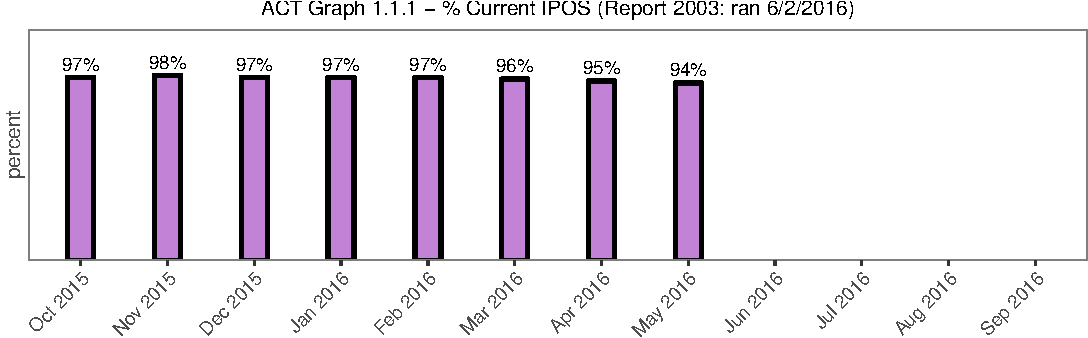
\includegraphics[width=\maxwidth]{figure/ACT_hist-1} 

\end{knitrout}

\begin{minipage}{\linewidth} { ACT: IPOS Table 1.1.1 \newline } % latex table generated in R 3.2.5 by xtable 1.8-2 package
% Thu Jun 02 15:32:37 2016
\scalebox{0.8}{
\begin{tabular}{p{0.10 \textwidth}|p{0.08 \textwidth}p{0.14 \textwidth}p{0.08 \textwidth}}
  \toprule
\textbf{month} & \textbf{current IPOS} & \textbf{blank/missing IPOS} & \textbf{expired IPOS} \\ 
  \midrule
Oct 2015 & 114 &   0 &   3 \\ 
  Nov 2015 & 116 &   0 &   2 \\ 
  Dec 2015 & 117 &   0 &   4 \\ 
   \rowcolor[gray]{0.90}Jan 2016 & 116 &   0 &   3 \\ 
   \rowcolor[gray]{0.90}Feb 2016 & 113 &   0 &   4 \\ 
   \rowcolor[gray]{0.90}Mar 2016 & 110 &   0 &   5 \\ 
  Apr 2016 & 108 &   0 &   6 \\ 
  May 2016 & 106 &   0 &   7 \\ 
   \bottomrule
\end{tabular}
}
 \par \bigskip \end{minipage}

\begin{minipage}{\linewidth} { ACT: IPOS Table 1.1.2 \newline } % latex table generated in R 3.2.5 by xtable 1.8-2 package
% Thu Jun 02 15:32:37 2016
\scalebox{0.8}{
\begin{tabular}{p{0.1\textwidth}|p{0.07\textwidth}p{0.07\textwidth}p{0.14 \textwidth}p{0.14\textwidth}p{0.15\textwidth}|p{0.08\textwidth}}
  \toprule
\textbf{month} & \textbf{Full IPOS} & \textbf{Interim IPOS} & \textbf{Interim IPOS Over 30 Days} & \textbf{Preliminary IPOS} & \textbf{Single Service IPOS} & \textbf{Grand Total} \\ 
  \midrule
Oct 2015 & 116 &   0 &   0 &   1 &   0 & 117 \\ 
  Nov 2015 & 117 &   1 &   0 &   0 &   0 & 118 \\ 
  Dec 2015 & 121 &  &   0 &  &  & 121 \\ 
   \rowcolor[gray]{0.90}Jan 2016 & 119 &  &   0 &  &  & 119 \\ 
   \rowcolor[gray]{0.90}Feb 2016 & 117 &  &   0 &  &  & 117 \\ 
   \rowcolor[gray]{0.90}Mar 2016 & 115 &  &   0 &  &  & 115 \\ 
  Apr 2016 & 112 &  &   0 &   1 &   1 & 114 \\ 
  May 2016 & 111 &  &   0 &   2 &  & 113 \\ 
   \bottomrule
\end{tabular}
}
 \par \bigskip \end{minipage}

\begin{minipage}{\linewidth} { ACT: IPOS Table 1.1.3 \newline } % latex table generated in R 3.2.5 by xtable 1.8-2 package
% Thu Jun 02 15:32:37 2016
\scalebox{0.8}{
\begin{tabular}{p{0.15\textwidth}|p{0.15\textwidth}p{0.25\textwidth}}
  \toprule
\textbf{supervisor} & \textbf{primary staff} & \textbf{expired/missing IPOS} \\ 
  \midrule
\textbf{Gentz, Lisa} &  & \hspace{2cm}\textbf{\textbf{1}} \\ 
   & Rahn, Nathan & 1 \\ 
  \textbf{Rahn, Nathan} &  & \hspace{2cm}\textbf{\textbf{6}} \\ 
   \rowcolor[gray]{0.90} & Behm, Emily & 1 \\ 
   \rowcolor[gray]{0.90} & Cunningham, Matthew & 5 \\ 
   \bottomrule
\end{tabular}
}
 \par \bigskip \end{minipage}

\begin{absolutelynopagebreak}
\subsection{Unsigned/Draft Documents}
\begin{knitrout}
\definecolor{shadecolor}{rgb}{0.969, 0.969, 0.969}\color{fgcolor}
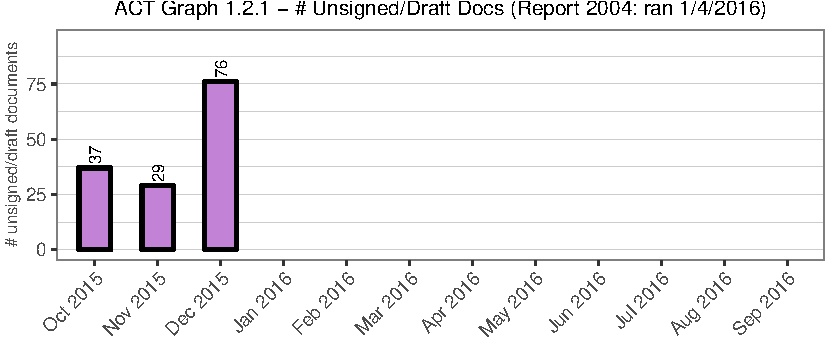
\includegraphics[width=\maxwidth]{figure/ACT_p_unsign-1} 

\end{knitrout}
\end{absolutelynopagebreak}

%' \begin{absolutelynopagebreak}
%' \subsection{Demographic Errors}
%' <<ACT_p_demo, fig.show="hold", message=FALSE, echo=FALSE, fig.height=2.25, fig.width=5.5>>=
%' p_demo$ACT
%' @
%' \end{absolutelynopagebreak}

%' \begin{absolutelynopagebreak}
%' \subsection{Health Errors}
%' <<ACT_p_health, fig.show="hold", message=FALSE, echo=FALSE, fig.height=2.25, fig.width=5.5>>=
%' p_health$ACT
%' @
%' \end{absolutelynopagebreak}

%' \begin{absolutelynopagebreak}
%' \subsection{Minimum Wage Errors}
%' <<ACT_p_wage, fig.show="hold", message=FALSE, echo=FALSE, fig.height=2.25, fig.width=5.5>>=
%' p_wage$ACT
%' @
%' \end{absolutelynopagebreak}

%%%%%%%%% CHILDREN'S SERVICES %%%%%%%%%%%%%%%%%%%%%%%%%%%%%%%%
% \begin{absolutelynopagebreak}
\section{Children's Services}
\subsection{IPOS}
\begin{knitrout}
\definecolor{shadecolor}{rgb}{0.969, 0.969, 0.969}\color{fgcolor}
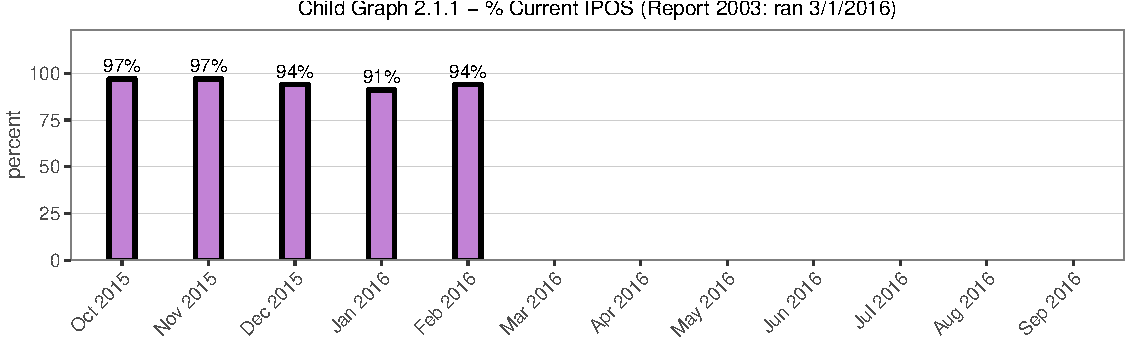
\includegraphics[width=\maxwidth]{figure/child_hist-1} 

\end{knitrout}
% \end{absolutelynopagebreak}

\begin{minipage}{\linewidth} { Children's Services: IPOS Table 2.1.1 \newline } % latex table generated in R 3.2.5 by xtable 1.8-2 package
% Thu Jun 02 15:32:38 2016
\scalebox{0.8}{
\begin{tabular}{p{0.10 \textwidth}|p{0.08 \textwidth}p{0.14 \textwidth}p{0.08 \textwidth}}
  \toprule
\textbf{month} & \textbf{current IPOS} & \textbf{blank/missing IPOS} & \textbf{expired IPOS} \\ 
  \midrule
Oct 2015 & 525 &   0 &  16 \\ 
  Nov 2015 & 527 &   0 &  16 \\ 
  Dec 2015 & 515 &   0 &  29 \\ 
   \rowcolor[gray]{0.90}Jan 2016 & 503 &   0 &  49 \\ 
   \rowcolor[gray]{0.90}Feb 2016 & 524 &   0 &  31 \\ 
   \rowcolor[gray]{0.90}Mar 2016 & 540 &   0 &  23 \\ 
  Apr 2016 & 540 &   0 &  33 \\ 
  May 2016 & 541 &   0 &  42 \\ 
   \bottomrule
\end{tabular}
}
 \par \bigskip \end{minipage}

\begin{minipage}{\linewidth} { Children's Services: IPOS Table 2.1.2 \newline } % latex table generated in R 3.2.5 by xtable 1.8-2 package
% Thu Jun 02 15:32:38 2016
\scalebox{0.8}{
\begin{tabular}{p{0.1\textwidth}|p{0.07\textwidth}p{0.07\textwidth}p{0.14\textwidth}p{0.14\textwidth}p{0.15\textwidth}|p{0.08\textwidth}}
  \toprule
\textbf{month} & \textbf{Full IPOS} & \textbf{Interim IPOS} & \textbf{Interim IPOS Over 30 Days} & \textbf{Preliminary IPOS} & \textbf{Single Service IPOS} & \textbf{Grand Total} \\ 
  \midrule
Oct 2015 & 508 &   1 &   0 &  32 &   0 & 541 \\ 
  Nov 2015 & 510 &   1 &   0 &  32 &   0 & 543 \\ 
  Dec 2015 & 509 &   1 &   0 &  34 &  & 544 \\ 
   \rowcolor[gray]{0.90}Jan 2016 & 508 &   1 &   1 &  43 &  & 552 \\ 
   \rowcolor[gray]{0.90}Feb 2016 & 522 &   1 &   0 &  32 &  & 555 \\ 
   \rowcolor[gray]{0.90}Mar 2016 & 519 &   1 &   1 &  43 &  & 563 \\ 
  Apr 2016 & 527 &   1 &   1 &  45 &  & 573 \\ 
  May 2016 & 538 &   7 &   1 &  38 &  & 583 \\ 
   \bottomrule
\end{tabular}
}
 \par \bigskip \end{minipage}

\begin{minipage}{\linewidth} { Children's Services: IPOS Table 2.1.3 \newline } % latex table generated in R 3.2.5 by xtable 1.8-2 package
% Thu Jun 02 15:32:38 2016
\scalebox{0.8}{
\begin{tabular}{p{0.18\textwidth}|p{0.20\textwidth}p{0.25\textwidth}}
  \toprule
\textbf{supervisor} & \textbf{primary staff} & \textbf{expired/missing IPOS} \\ 
  \midrule
\textbf{Bellus, Kelly} &  & \hspace{2cm}\textbf{\textbf{2}} \\ 
   & Hampton, Marlena & 2 \\ 
  \textbf{Brookens-Harvey, Barbara} &  & \hspace{2cm}\textbf{\textbf{4}} \\ 
   \rowcolor[gray]{0.90} & Hill, Mikki & 1 \\ 
   \rowcolor[gray]{0.90} & Lafeldt, Jennifer & 1 \\ 
   \rowcolor[gray]{0.90} & Mathison, Shannon & 1 \\ 
   & Womack, Nicole & 1 \\ 
  \textbf{Hapeman, Christine} &  & \hspace{2cm}\textbf{\textbf{30}} \\ 
   & Burnett, Karen & 5 \\ 
   \rowcolor[gray]{0.90} & Ferguson, Peter & 8 \\ 
   \rowcolor[gray]{0.90} & Fortune, Barbara & 10 \\ 
   \rowcolor[gray]{0.90} & Gray-Van Buren, Kelly & 2 \\ 
   & Jennings, Margaret & 4 \\ 
   & Rivest, Christina & 1 \\ 
  \textbf{LeVar, Sarah} &  & \hspace{2cm}\textbf{\textbf{10}} \\ 
   \rowcolor[gray]{0.90} & Hall, Philip & 4 \\ 
   \rowcolor[gray]{0.90} & Leadford, Elizabeth & 2 \\ 
   \rowcolor[gray]{0.90} & Perez, Irene & 1 \\ 
   & Starr, Catherine & 1 \\ 
   & Thurman, Judith & 2 \\ 
   \bottomrule
\end{tabular}
}
 \par \bigskip \end{minipage}

\begin{absolutelynopagebreak}
\subsection{Unsigned/Draft Documents}
\begin{knitrout}
\definecolor{shadecolor}{rgb}{0.969, 0.969, 0.969}\color{fgcolor}
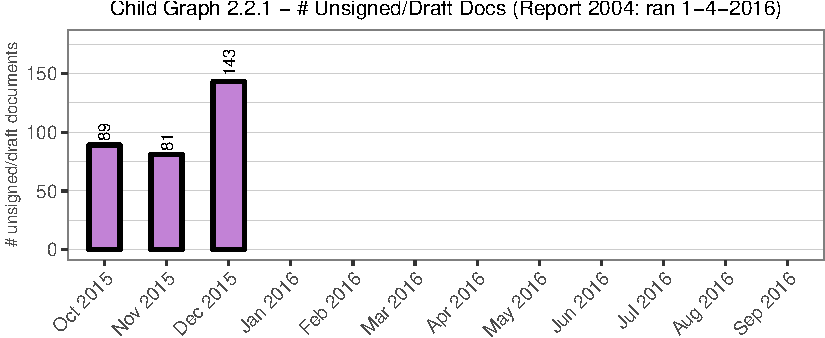
\includegraphics[width=\maxwidth]{figure/child_p_unsign-1} 

\end{knitrout}
\end{absolutelynopagebreak}

%' \begin{absolutelynopagebreak}
%' \subsection{Demographic Errors}
%' <<child_p_demo, fig.show="hold", message=FALSE, echo=FALSE, fig.height=2.25, fig.width=5.5>>=
%' p_demo$Child
%' @
%' \end{absolutelynopagebreak}

%' \begin{absolutelynopagebreak}
%' \subsection{Health Errors}
%' <<child_p_health, fig.show="hold", message=FALSE, echo=FALSE, fig.height=2.25, fig.width=5.5>>=
%' p_health$Child
%' @
%' \end{absolutelynopagebreak}

%' \begin{absolutelynopagebreak}
%' \subsection{Minimum Wage Errors}
%' <<child_p_wage, fig.show="hold", message=FALSE, echo=FALSE, fig.height=2.25, fig.width=5.5>>=
%' p_wage$Child
%' @
%' \end{absolutelynopagebreak}

%%%%%%%%%% Children's Services Home Based %%%%%%%%%%%%%%%%%%%
\pagebreak
\section{Children's Services Home Based}
\subsection{IPOS}
\begin{knitrout}
\definecolor{shadecolor}{rgb}{0.969, 0.969, 0.969}\color{fgcolor}
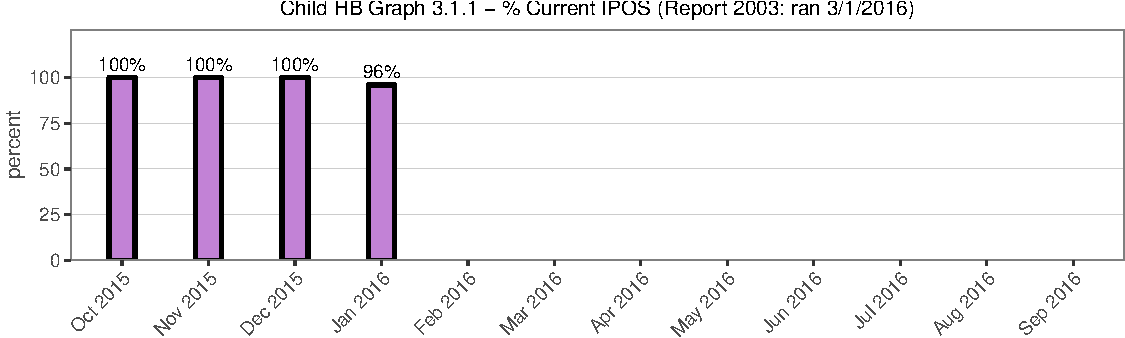
\includegraphics[width=\maxwidth]{figure/hb_hist-1} 

\end{knitrout}

\begin{minipage}{\linewidth} { Children's Services Home Based: IPOS Table 3.1.1 \newline } % latex table generated in R 3.2.5 by xtable 1.8-2 package
% Thu Jun 02 15:32:39 2016
\scalebox{0.8}{
\begin{tabular}{p{0.10 \textwidth}|p{0.08 \textwidth}p{0.14 \textwidth}p{0.08 \textwidth}}
  \toprule
\textbf{month} & \textbf{current IPOS} & \textbf{blank/missing IPOS} & \textbf{expired IPOS} \\ 
  \midrule
Oct 2015 &  27 &   0 &   0 \\ 
  Nov 2015 &  26 &   0 &   0 \\ 
  Dec 2015 &  23 &   0 &   0 \\ 
   \rowcolor[gray]{0.90}Jan 2016 &  22 &   0 &   1 \\ 
   \rowcolor[gray]{0.90}Feb 2016 &  21 &   0 &   0 \\ 
   \rowcolor[gray]{0.90}Mar 2016 &  23 &   0 &   0 \\ 
  Apr 2016 &  23 &   0 &   0 \\ 
  May 2016 &  19 &   0 &   1 \\ 
   \bottomrule
\end{tabular}
}
 \par \bigskip \end{minipage}

\begin{minipage}{\linewidth} { Children's Services Home Based: IPOS Table 3.1.2 \newline } % latex table generated in R 3.2.5 by xtable 1.8-2 package
% Thu Jun 02 15:32:39 2016
\scalebox{0.8}{
\begin{tabular}{p{0.1\textwidth}|p{0.07\textwidth}p{0.07\textwidth}p{0.14\textwidth}p{0.14\textwidth}p{0.15\textwidth}|p{0.08\textwidth}}
  \toprule
\textbf{month} & \textbf{Full IPOS} & \textbf{Interim IPOS} & \textbf{Interim IPOS Over 30 Days} & \textbf{Preliminary IPOS} & \textbf{Single Service IPOS} & \textbf{Grand Total} \\ 
  \midrule
Oct 2015 &  27 &   0 &   0 &   0 &   0 &  27 \\ 
  Nov 2015 &  26 &   0 &   0 &   0 &   0 &  26 \\ 
  Dec 2015 &  23 &  &   0 &  &  &  23 \\ 
   \rowcolor[gray]{0.90}Jan 2016 &  23 &  &   0 &  &  &  23 \\ 
   \rowcolor[gray]{0.90}Feb 2016 &  20 &  &   0 &   1 &  &  21 \\ 
   \rowcolor[gray]{0.90}Mar 2016 &  23 &  &   0 &  &  &  23 \\ 
  Apr 2016 &  23 &  &   0 &  &  &  23 \\ 
  May 2016 &  20 &  &   0 &  &  &  20 \\ 
   \bottomrule
\end{tabular}
}
 \par \bigskip \end{minipage}

\begin{minipage}{\linewidth} { Children's Services Home Based: IPOS Table 3.1.3 \newline } % latex table generated in R 3.2.5 by xtable 1.8-2 package
% Thu Jun 02 15:32:39 2016
\scalebox{0.8}{
\begin{tabular}{p{0.15\textwidth}|p{0.15\textwidth}p{0.25\textwidth}}
  \toprule
\textbf{supervisor} & \textbf{primary staff} & \textbf{expired/missing IPOS} \\ 
  \midrule
\textbf{Brookens-Harvey, Barbara} &  & \hspace{2cm}\textbf{\textbf{1}} \\ 
   & Womack, Nicole & 1 \\ 
   \bottomrule
\end{tabular}
}
 \par \bigskip \end{minipage}

\begin{absolutelynopagebreak}
\subsection{Unsigned/Draft Documents}
\begin{knitrout}
\definecolor{shadecolor}{rgb}{0.969, 0.969, 0.969}\color{fgcolor}
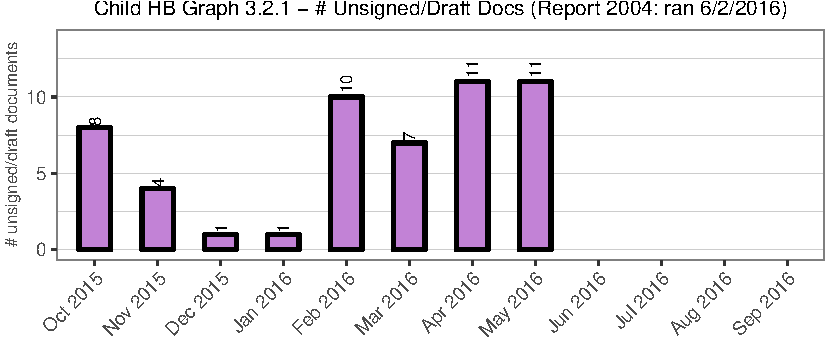
\includegraphics[width=\maxwidth]{figure/hb_p_unsign-1} 

\end{knitrout}
\end{absolutelynopagebreak}

%' \begin{absolutelynopagebreak}
%' \subsection{Demographic Errors}
%' <<hb_p_demo, fig.show="hold", message=FALSE, echo=FALSE, fig.height=2.25, fig.width=5.5>>=
%' p_demo$`Child HB`
%' @
%' \end{absolutelynopagebreak}

%' \begin{absolutelynopagebreak}
%' \subsection{Health Errors}
%' <<hb_p_health, fig.show="hold", message=FALSE, echo=FALSE, fig.height=2.25, fig.width=5.5>>=
%' p_health`Child HB`
%' @
%' \end{absolutelynopagebreak}

%%%%%%%%%% DD Adult %%%%%%%%%%%%%%%%%%%%%%
\pagebreak
\section{DD Adult}
\subsection{IPOS}
\begin{knitrout}
\definecolor{shadecolor}{rgb}{0.969, 0.969, 0.969}\color{fgcolor}
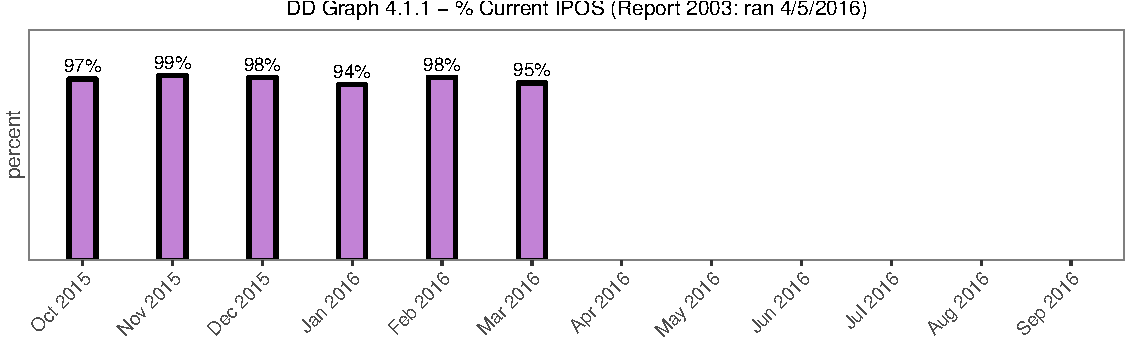
\includegraphics[width=\maxwidth]{figure/dd_hist-1} 

\end{knitrout}

\begin{minipage}{\linewidth} { DD Adult: IPOS Table 4.1.1 \newline } % latex table generated in R 3.2.5 by xtable 1.8-2 package
% Thu Jun 02 15:32:39 2016
\scalebox{0.8}{
\begin{tabular}{p{0.10 \textwidth}|p{0.08 \textwidth}p{0.14 \textwidth}p{0.08 \textwidth}}
  \toprule
\textbf{month} & \textbf{current IPOS} & \textbf{blank/missing IPOS} & \textbf{expired IPOS} \\ 
  \midrule
Oct 2015 & 892 &   0 &  31 \\ 
  Nov 2015 & 921 &   0 &  10 \\ 
  Dec 2015 & 918 &   0 &  14 \\ 
   \rowcolor[gray]{0.90}Jan 2016 & 875 &   0 &  57 \\ 
   \rowcolor[gray]{0.90}Feb 2016 & 912 &   0 &  20 \\ 
   \rowcolor[gray]{0.90}Mar 2016 & 880 &   0 &  44 \\ 
  Apr 2016 & 885 &   0 &  46 \\ 
  May 2016 & 878 &   0 &  58 \\ 
   \bottomrule
\end{tabular}
}
 \par \bigskip \end{minipage}

\begin{minipage}{\linewidth} { DD Adult: IPOS Table 4.1.2 \newline } % latex table generated in R 3.2.5 by xtable 1.8-2 package
% Thu Jun 02 15:32:39 2016
\scalebox{0.8}{
\begin{tabular}{p{0.1\textwidth}|p{0.07\textwidth}p{0.07\textwidth}p{0.14\textwidth}p{0.14\textwidth}p{0.15\textwidth}|p{0.08\textwidth}}
  \toprule
\textbf{month} & \textbf{Full IPOS} & \textbf{Interim IPOS} & \textbf{Interim IPOS Over 30 Days} & \textbf{Preliminary IPOS} & \textbf{Single Service IPOS} & \textbf{Grand Total} \\ 
  \midrule
Oct 2015 & 896 &  10 &   1 &   6 &  11 & 923 \\ 
  Nov 2015 & 901 &  10 &   1 &   9 &  11 & 931 \\ 
  Dec 2015 & 903 &   9 &   1 &   8 &  12 & 932 \\ 
   \rowcolor[gray]{0.90}Jan 2016 & 903 &  10 &   1 &   7 &  12 & 932 \\ 
   \rowcolor[gray]{0.90}Feb 2016 & 905 &  10 &   1 &   6 &  11 & 932 \\ 
   \rowcolor[gray]{0.90}Mar 2016 & 897 &  14 &   1 &   4 &   9 & 924 \\ 
  Apr 2016 & 892 &  19 &   4 &  10 &  10 & 931 \\ 
  May 2016 & 894 &  21 &   7 &  13 &   8 & 936 \\ 
   \bottomrule
\end{tabular}
}
 \par \bigskip \end{minipage}

\begin{minipage}{\linewidth} { DD Adult: IPOS Table 4.1.3 \newline } % latex table generated in R 3.2.5 by xtable 1.8-2 package
% Thu Jun 02 15:32:40 2016
\scalebox{0.8}{
\begin{tabular}{p{0.15\textwidth}|p{0.25\textwidth}p{0.25\textwidth}}
  \toprule
\textbf{supervisor} & \textbf{primary staff} & \textbf{expired/missing IPOS} \\ 
  \midrule
\textbf{Diephuis, Krista} &  & \hspace{2cm}\textbf{\textbf{1}} \\ 
   & Wells, Tracy & 1 \\ 
  \textbf{Dronamraju, Rani} &  & \hspace{2cm}\textbf{\textbf{20}} \\ 
   \rowcolor[gray]{0.90} & Bryant, Biancia & 1 \\ 
   \rowcolor[gray]{0.90} & Fenner, Caryette & 4 \\ 
   \rowcolor[gray]{0.90} & Kalina, Ernest & 2 \\ 
   & Klein, Jennifer & 4 \\ 
   & Lawson Chukwudi, Patricia & 4 \\ 
   & Price, Wendy & 2 \\ 
   \rowcolor[gray]{0.90} & Terry, Yvette & 1 \\ 
   \rowcolor[gray]{0.90} & Winston, Charles & 2 \\ 
   \rowcolor[gray]{0.90}\textbf{Mohring, Kathleen} &  & \hspace{2cm}\textbf{\textbf{15}} \\ 
   & Erickson, Sara & 1 \\ 
   & Mackenzie, Deborah & 14 \\ 
  \textbf{Wells, Tracy} &  & \hspace{2cm}\textbf{\textbf{22}} \\ 
   \rowcolor[gray]{0.90} & Green, Laura & 4 \\ 
   \rowcolor[gray]{0.90} & Hoover, Danielle & 1 \\ 
   \rowcolor[gray]{0.90} & Jacobs, Kevin & 2 \\ 
   & Karm, Thomas & 1 \\ 
   & Molascon, Holly & 1 \\ 
   & Petty, Cheryl & 8 \\ 
   \rowcolor[gray]{0.90} & Rich, Janet & 1 \\ 
   \rowcolor[gray]{0.90} & Schramm, Joshua & 4 \\ 
   \bottomrule
\end{tabular}
}
 \par \bigskip \end{minipage}

\begin{absolutelynopagebreak}
\subsection{Unsigned/Draft Documents}
\begin{knitrout}
\definecolor{shadecolor}{rgb}{0.969, 0.969, 0.969}\color{fgcolor}
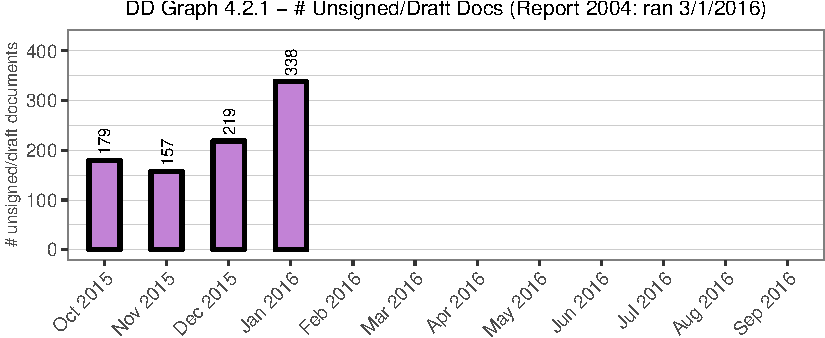
\includegraphics[width=\maxwidth]{figure/dd_p_unsign-1} 

\end{knitrout}
\end{absolutelynopagebreak}

%' \begin{absolutelynopagebreak}
%' \subsection{Demographic Errors}
%' <<dd_p_demo, fig.show="hold", message=FALSE, echo=FALSE, fig.height=2.25, fig.width=5.5>>=
%' p_demo$DD
%' @
%' \end{absolutelynopagebreak}

%' \begin{absolutelynopagebreak}
%' \subsection{Health Errors}
%' <<dd_p_health, fig.show="hold", message=FALSE, echo=FALSE, fig.height=2.25, fig.width=5.5>>=
%' p_health$DD
%' @
%' \end{absolutelynopagebreak}

%' % \begin{absolutelynopagebreak}
%' \subsection{Minimum Wage Errors}
%' <<dd_p_wage, fig.show="hold", message=FALSE, echo=FALSE, fig.height=2.25, fig.width=5.5>>=
%' p_wage$DD
%' @
%' % \end{absolutelynopagebreak}

%%%%%%%%%% MI Adult %%%%%%%%%%%%%%%%%%%%%
% \begin{absolutelynopagebreak}
\section{MI Adult}
\subsection{IPOS}
\begin{knitrout}
\definecolor{shadecolor}{rgb}{0.969, 0.969, 0.969}\color{fgcolor}
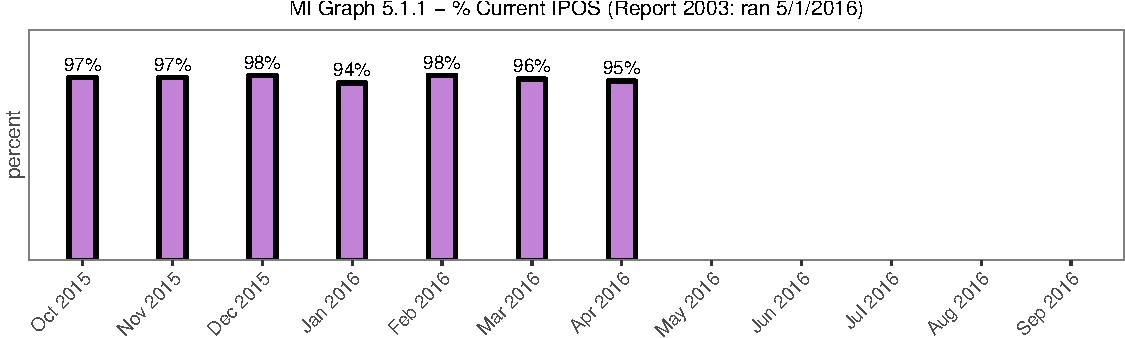
\includegraphics[width=\maxwidth]{figure/mi_hist-1} 

\end{knitrout}
% \end{absolutelynopagebreak}

\begin{minipage}{\linewidth} { MI Adult: IPOS Table 5.1.1 \newline } % latex table generated in R 3.2.5 by xtable 1.8-2 package
% Thu Jun 02 15:32:40 2016
\scalebox{0.8}{
\begin{tabular}{p{0.10 \textwidth}|p{0.08 \textwidth}p{0.14 \textwidth}p{0.08 \textwidth}}
  \toprule
\textbf{month} & \textbf{current IPOS} & \textbf{blank/missing IPOS} & \textbf{expired IPOS} \\ 
  \midrule
Oct 2015 & 1750 &   0 &  59 \\ 
  Nov 2015 & 1744 &   0 &  50 \\ 
  Dec 2015 & 1755 &   0 &  42 \\ 
   \rowcolor[gray]{0.90}Jan 2016 & 1682 &   0 & 106 \\ 
   \rowcolor[gray]{0.90}Feb 2016 & 1742 &   0 &  39 \\ 
   \rowcolor[gray]{0.90}Mar 2016 & 1682 &   0 &  64 \\ 
  Apr 2016 & 1682 &   0 &  79 \\ 
  May 2016 & 1689 &   0 &  80 \\ 
   \bottomrule
\end{tabular}
}
 \par \bigskip \end{minipage}

\begin{minipage}{\linewidth} { MI Adult: IPOS Table 5.1.2 \newline } % latex table generated in R 3.2.5 by xtable 1.8-2 package
% Thu Jun 02 15:32:40 2016
\scalebox{0.8}{
\begin{tabular}{p{0.1\textwidth}|p{0.07\textwidth}p{0.07\textwidth}p{0.14\textwidth}p{0.14\textwidth}p{0.15\textwidth}|p{0.08\textwidth}}
  \toprule
\textbf{month} & \textbf{Full IPOS} & \textbf{Interim IPOS} & \textbf{Interim IPOS Over 30 Days} & \textbf{Preliminary IPOS} & \textbf{Single Service IPOS} & \textbf{Grand Total} \\ 
  \midrule
Oct 2015 & 1756 &   2 &   1 &  48 &   3 & 1809 \\ 
  Nov 2015 & 1740 &   6 &   2 &  45 &   3 & 1794 \\ 
  Dec 2015 & 1741 &  15 &   6 &  38 &   3 & 1797 \\ 
   \rowcolor[gray]{0.90}Jan 2016 & 1736 &  14 &   8 &  35 &   3 & 1788 \\ 
   \rowcolor[gray]{0.90}Feb 2016 & 1734 &   7 &   3 &  36 &   4 & 1781 \\ 
   \rowcolor[gray]{0.90}Mar 2016 & 1696 &   8 &   4 &  39 &   3 & 1746 \\ 
  Apr 2016 & 1706 &   6 &   3 &  43 &   6 & 1761 \\ 
  May 2016 & 1700 &  13 &  11 &  52 &   4 & 1769 \\ 
   \bottomrule
\end{tabular}
}
 \par \bigskip \end{minipage}

% latex table generated in R 3.2.5 by xtable 1.8-2 package
% Thu Jun 02 15:32:40 2016
\begin{longtable} { >{\raggedright}p{0.14\textwidth}|p{0.30\textwidth}p{0.25\textwidth}}
  \multicolumn{3}{l}{{MI Adult: IPOS Table 5.1.3}}\ \label{}\\  \toprule  \textbf{supervisor}  & \textbf{primary staff} & \textbf{expired/missing IPOS} \\\midrule  \endfirsthead  \multicolumn{3}{c}{{MI Adult: IPOS Table 5.1.3 -- continued from previous page}}\\  \toprule  \textbf{supervisor} & \textbf{primary staff}& \textbf{expired/missing IPOS} \\\midrule  \endhead  \midrule  \multicolumn{3}{r}{{Continued on next page}}\\  \bottomrule \endfoot  \bottomrule \endlastfoot  \textbf{Edwards, Sheri} &  & \hspace{2cm}\textbf{\textbf{17}} \\ 
   & Allen, Katekia & 2 \\ 
   & Donald, Angela & 3 \\ 
   \rowcolor[gray]{0.90} & Jordan, Shad & 1 \\ 
   \rowcolor[gray]{0.90} & Jung, Kayla & 2 \\ 
   \rowcolor[gray]{0.90} & McLemore, Sherry & 2 \\ 
   & Perry, Meredith & 1 \\ 
   & Schoffner, Shamekia & 2 \\ 
   & Svensson, Kathy & 1 \\ 
   \rowcolor[gray]{0.90} & Toole, Keisha & 3 \\ 
   \rowcolor[gray]{0.90}\textbf{Gentz, Judith} &  & \hspace{2cm}\textbf{\textbf{1}} \\ 
   \rowcolor[gray]{0.90} & Meadows, Cassandra & 1 \\ 
  \textbf{Halliday, Jessica} &  & \hspace{2cm}\textbf{\textbf{17}} \\ 
   & Bajema, Stacey & 4 \\ 
   & Beckley, Jeff & 4 \\ 
   \rowcolor[gray]{0.90} & Johnson, Tamika & 1 \\ 
   \rowcolor[gray]{0.90} & Melody, Alex & 4 \\ 
   \rowcolor[gray]{0.90} & O'Donnell, Alexandra & 3 \\ 
   & Thomas, Kristian & 1 \\ 
  \textbf{Hoener, Katie} &  & \hspace{2cm}\textbf{\textbf{5}} \\ 
   & Lampe, Mary & 2 \\ 
   \rowcolor[gray]{0.90} & Montgomery, Ebony & 1 \\ 
   \rowcolor[gray]{0.90} & Twigg, Scott & 2 \\ 
   \rowcolor[gray]{0.90}\textbf{Lembesis (Stanton), Jennifer} &  & \hspace{2cm}\textbf{\textbf{17}} \\ 
   & Davis, Shauntai & 6 \\ 
   & Haver, Shanna & 2 \\ 
   & Miron, Jason & 2 \\ 
   \rowcolor[gray]{0.90} & Reid, Courtney & 7 \\ 
   \rowcolor[gray]{0.90}\textbf{Noe, Tori} &  & \hspace{2cm}\textbf{\textbf{1}} \\ 
   \rowcolor[gray]{0.90} & Ray, Pamela & 1 \\ 
  \textbf{Shovels, John} &  & \hspace{2cm}\textbf{\textbf{2}} \\ 
   & Edwards, Sheri & 1 \\ 
   & Stacy, John & 1 \\ 
   \rowcolor[gray]{0.90}\textbf{Stacy, John} &  & \hspace{2cm}\textbf{\textbf{21}} \\ 
   \rowcolor[gray]{0.90} & Batzer, Stacey & 5 \\ 
   \rowcolor[gray]{0.90} & Blach, Aura & 5 \\ 
   & Martin, Kelly & 2 \\ 
   & Noe, Tori & 1 \\ 
   & Reina, Aaron & 4 \\ 
   \rowcolor[gray]{0.90} & Sims, Elaina & 4 \\ 
   \end{longtable}


\begin{absolutelynopagebreak}
\subsection{Unsigned/Draft Documents}
\begin{knitrout}
\definecolor{shadecolor}{rgb}{0.969, 0.969, 0.969}\color{fgcolor}
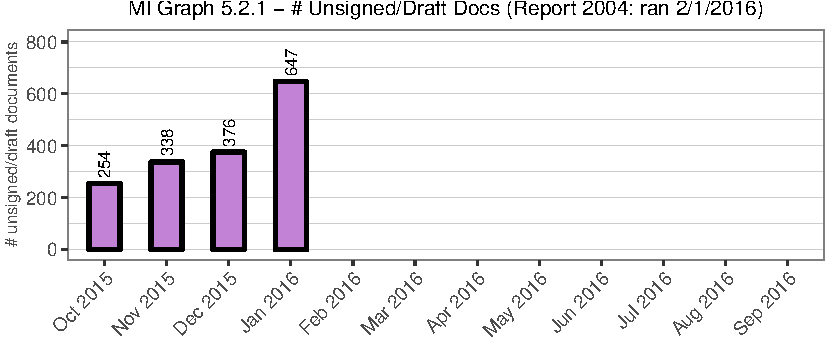
\includegraphics[width=\maxwidth]{figure/mi_p_unsign-1} 

\end{knitrout}
\end{absolutelynopagebreak}

%' \begin{absolutelynopagebreak}
%' \subsection{Demographic Errors}
%' <<mi_p_demo, fig.show="hold", message=FALSE, echo=FALSE, fig.height=2.25, fig.width=5.5>>=
%' p_demo$MI
%' @
%' \end{absolutelynopagebreak}

%' \subsection{Health Errors}
%' <<mi_p_health, fig.show="hold", message=FALSE, echo=FALSE, fig.height=2.25, fig.width=5.5>>=
%' p_health$MI
%' @

%' \begin{absolutelynopagebreak}
%' \subsection{Minimum Wage Errors}
%' <<mi_p_wage, fig.show="hold", message=FALSE, echo=FALSE, fig.height=2.25, fig.width=5.5>>=
%' p_wage$MI
%' @
%' \end{absolutelynopagebreak}

\pagebreak
\section{Unsigned and Draft Documents}
\small{
% latex table generated in R 3.2.5 by xtable 1.8-2 package
% Thu Jun 02 15:32:41 2016
\begin{longtable} { >{\raggedright}p{0.25\textwidth}|p{0.27\textwidth}p{0.22\textwidth}}
  \multicolumn{3}{l}{{Table 6.1}}\ \label{}\\  \toprule  \textbf{supervisor}  & \textbf{author} & \textbf{unsigned/draft docs} \\\midrule  \endfirsthead  \multicolumn{3}{c}{{Table 6.1 -- continued from previous page}}\\  \toprule  \textbf{supervisor} & \textbf{author}& \textbf{unsigned/draft docs} \\\midrule  \endhead  \midrule  \multicolumn{3}{r}{{Continued on next page}}\\  \bottomrule \endfoot  \bottomrule \endlastfoot  \textbf{Auiler, Carol} &  & \hspace{2cm}\textbf{1} \\ 
   & Hillier, Skye & 1 \\ 
  \textbf{Benjamins, Mary} &  & \hspace{2cm}\textbf{2} \\ 
   \rowcolor[gray]{0.90} & Banks, LaSondra & 2 \\ 
   \rowcolor[gray]{0.90}\textbf{Bright, Jessica} &  & \hspace{2cm}\textbf{2} \\ 
   \rowcolor[gray]{0.90} & Natala, Nakita & 2 \\ 
  \textbf{Brookens-Harvey, Barbara} &  & \hspace{2cm}\textbf{55} \\ 
   & Burton, Alexia & 7 \\ 
   & Hill, Mikki & 1 \\ 
   \rowcolor[gray]{0.90} & Leimstoll, Dawn & 36 \\ 
   \rowcolor[gray]{0.90} & Mathison, Shannon & 3 \\ 
   \rowcolor[gray]{0.90} & McClure, Eric & 5 \\ 
   & Womack, Nicole & 3 \\ 
  \textbf{Chisholm, Debra} &  & \hspace{2cm}\textbf{42} \\ 
   & Patterson, Kiarra & 1 \\ 
   \rowcolor[gray]{0.90} & Philpot, Mary & 9 \\ 
   \rowcolor[gray]{0.90} & Rankin, Linnae & 1 \\ 
   \rowcolor[gray]{0.90} & Seldon, Kyesa & 1 \\ 
   & Smith, Irene & 4 \\ 
   & Thomas, Lucille & 22 \\ 
   & Weems, William & 1 \\ 
   \rowcolor[gray]{0.90} & Wilson, Mike & 3 \\ 
   \rowcolor[gray]{0.90}\textbf{Cortes, Patricia} &  & \hspace{2cm}\textbf{6} \\ 
   \rowcolor[gray]{0.90} & Diephuis, Krista & 1 \\ 
   & Florence, Timothy & 4 \\ 
   & Spring, Elizabeth & 1 \\ 
  \textbf{Darling, Gerri} &  & \hspace{2cm}\textbf{2} \\ 
   \rowcolor[gray]{0.90} & Student1, RN & 1 \\ 
   \rowcolor[gray]{0.90} & Student6, RN & 1 \\ 
   \rowcolor[gray]{0.90}\textbf{Diephuis, Krista} &  & \hspace{2cm}\textbf{2} \\ 
   & Gilkey, Jenoah & 1 \\ 
   & Wells, Tracy & 1 \\ 
  \textbf{Dronamraju, Rani} &  & \hspace{2cm}\textbf{90} \\ 
   \rowcolor[gray]{0.90} & Ernst, Jessica & 6 \\ 
   \rowcolor[gray]{0.90} & Fenner, Caryette & 8 \\ 
   \rowcolor[gray]{0.90} & Kalina, Ernest & 2 \\ 
   & Klein, Jennifer & 6 \\ 
   & Lawson Chukwudi, Patricia & 22 \\ 
   & McClain, Ashley & 1 \\ 
   \rowcolor[gray]{0.90} & Price, Wendy & 3 \\ 
   \rowcolor[gray]{0.90} & Quine, Daniel & 2 \\ 
   \rowcolor[gray]{0.90} & Rathbun, Pam & 13 \\ 
   & Terry, Yvette & 7 \\ 
   & Trinka, Lisa & 1 \\ 
   & Winston, Charles & 7 \\ 
   \rowcolor[gray]{0.90} & Yu, Lucia & 12 \\ 
   \rowcolor[gray]{0.90}\textbf{Edwards, Sheri} &  & \hspace{2cm}\textbf{79} \\ 
   \rowcolor[gray]{0.90} & Allen, Katekia & 17 \\ 
   & Atwell, Andrea & 5 \\ 
   & Blaze, Renee & 1 \\ 
   & Donald, Angela & 4 \\ 
   \rowcolor[gray]{0.90} & Jordan, Shad & 10 \\ 
   \rowcolor[gray]{0.90} & Jung, Kayla & 1 \\ 
   \rowcolor[gray]{0.90} & McLemore, Sherry & 4 \\ 
   & Perry, Meredith & 1 \\ 
   & Schoffner, Shamekia & 23 \\ 
   & Svensson, Kathy & 11 \\ 
   \rowcolor[gray]{0.90} & Toole, Keisha & 2 \\ 
   \rowcolor[gray]{0.90}\textbf{Florence, Timothy} &  & \hspace{2cm}\textbf{416} \\ 
   \rowcolor[gray]{0.90} & Atkins, Thomas & 11 \\ 
   & Bright, Jessica & 25 \\ 
   & Demehri, Angela & 10 \\ 
   & Edwards, Lauren & 1 \\ 
   \rowcolor[gray]{0.90} & Gargan, Michele & 8 \\ 
   \rowcolor[gray]{0.90} & Gentz, Judith & 4 \\ 
   \rowcolor[gray]{0.90} & Hashimoto, Martha & 8 \\ 
   & Healy III, Daniel & 32 \\ 
   & Husby, Leah & 71 \\ 
   & Mayman, Daniel & 14 \\ 
   \rowcolor[gray]{0.90} & Mobilio, Andrea & 75 \\ 
   \rowcolor[gray]{0.90} & Shauger, Michelle & 12 \\ 
   \rowcolor[gray]{0.90} & Ssemanda, Elizabeth & 1 \\ 
   & Stetz, Sharon & 59 \\ 
   & Washington, W. Craig & 85 \\ 
  \textbf{Gentz, Lisa} &  & \hspace{2cm}\textbf{57} \\ 
   \rowcolor[gray]{0.90} & Leadford, William & 3 \\ 
   \rowcolor[gray]{0.90} & Rahn, Nathan & 52 \\ 
   \rowcolor[gray]{0.90} & Tasker, Melisa & 2 \\ 
  \textbf{Hagaman, Brandie} &  & \hspace{2cm}\textbf{12} \\ 
   & Achatz, Charles & 1 \\ 
   & Fellabaum, Kathleen & 3 \\ 
   \rowcolor[gray]{0.90} & Hershberger, Merton & 1 \\ 
   \rowcolor[gray]{0.90} & Lewis, Destiny & 1 \\ 
   \rowcolor[gray]{0.90} & O'brien, Colleen & 3 \\ 
   & Rama, Linda & 3 \\ 
  \textbf{Halliday, Jessica} &  & \hspace{2cm}\textbf{57} \\ 
   & Bajema, Stacey & 4 \\ 
   \rowcolor[gray]{0.90} & Beckley, Jeff & 6 \\ 
   \rowcolor[gray]{0.90} & Beland, Darren & 23 \\ 
   \rowcolor[gray]{0.90} & Hellenberg, Emily & 4 \\ 
   & Melody, Alex & 3 \\ 
   & O'Donnell, Alexandra & 5 \\ 
   & Thomas, Kristian & 7 \\ 
   \rowcolor[gray]{0.90} & Tisdale, Tina & 5 \\ 
   \rowcolor[gray]{0.90}\textbf{Hapeman, Christine} &  & \hspace{2cm}\textbf{52} \\ 
   \rowcolor[gray]{0.90} & Burnett, Karen & 1 \\ 
   & Fortune, Barbara & 30 \\ 
   & Gray-Van Buren, Kelly & 3 \\ 
   & Jennings, Margaret & 6 \\ 
   \rowcolor[gray]{0.90} & Rivest, Christina & 9 \\ 
   \rowcolor[gray]{0.90} & Sulfaro, Laura & 3 \\ 
   \rowcolor[gray]{0.90}\textbf{Healy III, Daniel} &  & \hspace{2cm}\textbf{2} \\ 
   & Wright, Paul & 2 \\ 
  \textbf{Hoener, Katie} &  & \hspace{2cm}\textbf{35} \\ 
   & Eggleston, Debra & 1 \\ 
   \rowcolor[gray]{0.90} & Lampe, Mary & 10 \\ 
   \rowcolor[gray]{0.90} & MacCormack, Catherine & 6 \\ 
   \rowcolor[gray]{0.90} & Mullaly, Margaret & 1 \\ 
   & Shaffer (Kniceley), Ashley & 9 \\ 
   & Twigg, Scott & 8 \\ 
  \textbf{Knapp, Timothy} &  & \hspace{2cm}\textbf{8} \\ 
   \rowcolor[gray]{0.90} & Ghedotte, Janette & 6 \\ 
   \rowcolor[gray]{0.90} & Pearson, Thomas & 2 \\ 
   \rowcolor[gray]{0.90}\textbf{LeVar, Sarah} &  & \hspace{2cm}\textbf{74} \\ 
   & Black, Janessa & 2 \\ 
   & Hall, Philip & 20 \\ 
   & Iekel-Johnson, Susan & 1 \\ 
   \rowcolor[gray]{0.90} & Leadford, Elizabeth & 17 \\ 
   \rowcolor[gray]{0.90} & Perez, Irene & 1 \\ 
   \rowcolor[gray]{0.90} & Starr, Catherine & 33 \\ 
  \textbf{Leadford, William} &  & \hspace{2cm}\textbf{33} \\ 
   & Badri, Soumaya & 9 \\ 
   & Barnes, Alesha & 2 \\ 
   \rowcolor[gray]{0.90} & Benton-Brown, Miayana & 1 \\ 
   \rowcolor[gray]{0.90} & Burchard, Angela & 1 \\ 
   \rowcolor[gray]{0.90} & Hyde, Hannah & 1 \\ 
   & Lloyd, Sylvia & 9 \\ 
   & Muraca, Nicole & 3 \\ 
   & Starkey, Sarah & 3 \\ 
   \rowcolor[gray]{0.90} & Stevenson, Jennifer & 4 \\ 
   \rowcolor[gray]{0.90}\textbf{Lembesis (Stanton), Jennifer} &  & \hspace{2cm}\textbf{61} \\ 
   \rowcolor[gray]{0.90} & Brouwer, Patricia & 3 \\ 
   & Davis, Shauntai & 23 \\ 
   & Grimes, Spring & 5 \\ 
   & Haver, Shanna & 4 \\ 
   \rowcolor[gray]{0.90} & Miron, Jason & 11 \\ 
   \rowcolor[gray]{0.90} & Reid, Courtney & 12 \\ 
   \rowcolor[gray]{0.90} & Rossman, Mary & 3 \\ 
  \textbf{Lovelace, Julie} &  & \hspace{2cm}\textbf{13} \\ 
   & Bagby, Chelsea & 13 \\ 
  \textbf{Mohring, Kathleen} &  & \hspace{2cm}\textbf{127} \\ 
   \rowcolor[gray]{0.90} & Auiler, Carol & 1 \\ 
   \rowcolor[gray]{0.90} & Axberg, Stephanie & 27 \\ 
   \rowcolor[gray]{0.90} & Erickson, Sara & 6 \\ 
   & Ferriter, Michael & 40 \\ 
   & Lovelace, Julie & 20 \\ 
   & Mackenzie, Deborah & 3 \\ 
   \rowcolor[gray]{0.90} & McMillon, Tracy & 18 \\ 
   \rowcolor[gray]{0.90} & Moore, Carmen & 3 \\ 
   \rowcolor[gray]{0.90} & Umholtz, Elaine & 7 \\ 
   & Wright, Christine & 2 \\ 
  \textbf{O'brien, Colleen} &  & \hspace{2cm}\textbf{21} \\ 
   & Bale, Melanie & 2 \\ 
   \rowcolor[gray]{0.90} & Farrow, Marlene & 3 \\ 
   \rowcolor[gray]{0.90} & Flanagan, Deborah & 14 \\ 
   \rowcolor[gray]{0.90} & Lancaster, Dea & 2 \\ 
  \textbf{Owen, Debra} &  & \hspace{2cm}\textbf{54} \\ 
   & Adkins, Douglas & 2 \\ 
   & Churchill, Amanda & 1 \\ 
   \rowcolor[gray]{0.90} & Dixon, Charlotte & 2 \\ 
   \rowcolor[gray]{0.90} & Hartman, LaShanda & 2 \\ 
   \rowcolor[gray]{0.90} & Kreager, Rebecca & 43 \\ 
   & Sommerville, Tomekia & 3 \\ 
   & Wilson, Terrance & 1 \\ 
  \textbf{Paxton, Britt} &  & \hspace{2cm}\textbf{31} \\ 
   \rowcolor[gray]{0.90} & Black, Devon & 2 \\ 
   \rowcolor[gray]{0.90} & Culberson, Warren & 6 \\ 
   \rowcolor[gray]{0.90} & Fails, Bonita & 1 \\ 
   & Kalluri, Usha & 18 \\ 
   & Prince, David & 1 \\ 
   & Willis, Keisha & 3 \\ 
   \rowcolor[gray]{0.90}\textbf{Rahn, Nathan} &  & \hspace{2cm}\textbf{234} \\ 
   \rowcolor[gray]{0.90} & Behm, Emily & 7 \\ 
   \rowcolor[gray]{0.90} & Burpee, Elena & 9 \\ 
   & Cunningham, Matthew & 86 \\ 
   & Ellis, Shannon & 13 \\ 
   & Goode, Casey & 21 \\ 
   \rowcolor[gray]{0.90} & Hoogerhyde, Jill & 26 \\ 
   \rowcolor[gray]{0.90} & Ing, Daniel & 21 \\ 
   \rowcolor[gray]{0.90} & Jabzanka, Thaddeus & 6 \\ 
   & Messina, Heather & 12 \\ 
   & Scott, Vivian & 1 \\ 
   & Srivastava, Sabreen & 11 \\ 
   \rowcolor[gray]{0.90} & Woodward, Devon & 21 \\ 
   \rowcolor[gray]{0.90}\textbf{Sattler, Lydia} &  & \hspace{2cm}\textbf{29} \\ 
   \rowcolor[gray]{0.90} & Farler, Corrie & 6 \\ 
   & Fish, Tara & 19 \\ 
   & Lawson, Kapra & 2 \\ 
   & Slocum, Deborah & 1 \\ 
   \rowcolor[gray]{0.90} & Vowels, Jill & 1 \\ 
   \rowcolor[gray]{0.90}\textbf{Schrader, Lisa} &  & \hspace{2cm}\textbf{17} \\ 
   \rowcolor[gray]{0.90} & Millar, Thana & 5 \\ 
   & Mitchell, Holly & 12 \\ 
  \textbf{Sheng, Mei-fu} &  & \hspace{2cm}\textbf{1} \\ 
   & Patania, Judith & 1 \\ 
   \rowcolor[gray]{0.90}\textbf{Shovels, John} &  & \hspace{2cm}\textbf{15} \\ 
   \rowcolor[gray]{0.90} & Edwards, Sheri & 5 \\ 
   \rowcolor[gray]{0.90} & Halliday, Jessica & 6 \\ 
   & Hoener, Katie & 2 \\ 
   & Stacy, John & 2 \\ 
  \textbf{Stacy, John} &  & \hspace{2cm}\textbf{32} \\ 
   \rowcolor[gray]{0.90} & Batzer, Stacey & 2 \\ 
   \rowcolor[gray]{0.90} & Blach, Aura & 1 \\ 
   \rowcolor[gray]{0.90} & Lewis, Andrew & 4 \\ 
   & Martin, Kelly & 8 \\ 
   & Michalowski, Bryan & 3 \\ 
   & Ruggeberg (Wolters), Lisa & 2 \\ 
   \rowcolor[gray]{0.90} & Sims, Elaina & 12 \\ 
   \rowcolor[gray]{0.90}\textbf{Stearns, Stephanie} &  & \hspace{2cm}\textbf{8} \\ 
   \rowcolor[gray]{0.90} & Pickard, Steven & 8 \\ 
  \textbf{Tasker, Melisa} &  & \hspace{2cm}\textbf{9} \\ 
   & Watson, Tia & 9 \\ 
  \textbf{Wells, Tracy} &  & \hspace{2cm}\textbf{45} \\ 
   \rowcolor[gray]{0.90} & Dooley, Mary & 5 \\ 
   \rowcolor[gray]{0.90} & Fillman-Hatcher, Carolyn & 1 \\ 
   \rowcolor[gray]{0.90} & Green, Laura & 5 \\ 
   & Hoover, Danielle & 2 \\ 
   & Jacobs, Sarah & 1 \\ 
   & Karm, Thomas & 1 \\ 
   \rowcolor[gray]{0.90} & Petty, Cheryl & 4 \\ 
   \rowcolor[gray]{0.90} & Pickrel, April & 2 \\ 
   \rowcolor[gray]{0.90} & Schramm, Joshua & 23 \\ 
   & Traverse, Laura & 1 \\ 
  \textbf{NA} &  & \hspace{2cm}\textbf{1} \\ 
   & Johnson, Christina & 1 \\ 
   \rowcolor[gray]{0.90}\textbf{Grand total} &  & \textbf{1725} \\ 
   \end{longtable}

}

\pagebreak

\section{Caseload and Not Seen 30/60/90/180 days}
Caseload and Not Seen 30/60/90/180 days (No services at all) \newline
\small{
% latex table generated in R 3.2.5 by xtable 1.8-2 package
% Thu Jun 02 15:32:41 2016
\begin{longtable} { >{\raggedright}p{0.05\textwidth}p{0.22\textwidth}p{0.05\textwidth}p{0.09\textwidth}p{0.09\textwidth}p{0.09\textwidth}p{0.09\textwidth}p{0.09\textwidth}}
  \multicolumn{8}{l}{{Table 6.1}}\ \label{}\\  \toprule  \textbf{team}  & \textbf{primary staff} & \textbf{case load} & \textbf{level} & \textbf{days $>$ 30} & \textbf{days $>$ 60} & \textbf{days $>$ 90} & \textbf{days $>$ 180} \\\midrule  \endfirsthead  \multicolumn{8}{c}{{Table 6.1 -- continued from previous page}}\\  \toprule  \textbf{team} & \textbf{primary staff}& \textbf{case load}& \textbf{level}& \textbf{days $>$ 30}& \textbf{days $>$ 60}& \textbf{days $>$ 90}& \textbf{days $>$ 180} \\\midrule  \endhead  \midrule  \multicolumn{8}{r}{{Continued on next page}}\\  \bottomrule \endfoot  \bottomrule \endlastfoot  \textbf{ACT Team} &  & \textbf{113} & - & \textbf{17} & \textbf{8} & \textbf{5} & \textbf{1} \\ 
   & Behm, Emily & 22 & 4 & 5 & 2 & 0 & 0 \\ 
   & Cunningham, Matthew & 16 & 4 & 4 & 2 & 2 & 1 \\ 
   \rowcolor[gray]{0.90} & Ellis, Shannon & 1 & 4 & 0 & 0 & 0 & 0 \\ 
   \rowcolor[gray]{0.90} & Hellenberg, Emily & 5 & 4 & 0 & 0 & 0 & 0 \\ 
   \rowcolor[gray]{0.90} & Ing, Daniel & 10 & 4 & 2 & 2 & 1 & 0 \\ 
   & Messina, Heather & 11 & 4 & 2 & 0 & 0 & 0 \\ 
   & Rahn, Nathan & 9 & 4 & 1 & 0 & 0 & 0 \\ 
   & Srivastava, Sabreen & 22 & 4 & 2 & 2 & 2 & 0 \\ 
   \rowcolor[gray]{0.90} & Twigg, Scott & 1 & 4 & 0 & 0 & 0 & 0 \\ 
   \rowcolor[gray]{0.90} & Woodward, Devon & 16 & 4 & 1 & 0 & 0 & 0 \\ 
   \hline
\textbf{Child} &  & \textbf{579} & - & \textbf{269} & \textbf{151} & \textbf{70} & \textbf{18} \\ 
   & Angeski-Barron, Michelle & 25 & 3 & 2 & 1 & 0 & 0 \\ 
   & Bauer, Ann & 5 & 3 & 5 & 4 & 4 & 4 \\ 
   & Black, Janessa & 28 & 3 & 14 & 6 & 2 & 0 \\ 
   \rowcolor[gray]{0.90} & Brookens-Harvey, Barbara & 3 & 3 & 1 & 0 & 0 & 0 \\ 
   \rowcolor[gray]{0.90} & Burnett, Karen & 34 & 3 & 12 & 9 & 5 & 0 \\ 
   \rowcolor[gray]{0.90} & Burton, Alexia & 12 & 3 & 5 & 3 & 2 & 1 \\ 
   & Depp, John & 28 & 3 & 14 & 6 & 1 & 0 \\ 
   & Ellis, Shannon & 1 & 3 & 0 & 0 & 0 & 0 \\ 
   & Ferguson, Peter & 51 & 3 & 33 & 25 & 10 & 2 \\ 
   \rowcolor[gray]{0.90} & Fortune, Barbara & 32 & 3 & 23 & 21 & 14 & 5 \\ 
   \rowcolor[gray]{0.90} & Gray-Van Buren, Kelly & 28 & 3 & 18 & 6 & 2 & 0 \\ 
   \rowcolor[gray]{0.90} & Hall, Philip & 30 & 3 & 12 & 8 & 5 & 1 \\ 
   & Hampton, Marlena & 3 & 3 & 3 & 0 & 0 & 0 \\ 
   & Hill, Mikki & 7 & 3 & 2 & 2 & 2 & 0 \\ 
   & Iekel-Johnson, Susan & 29 & 3 & 15 & 8 & 5 & 0 \\ 
   \rowcolor[gray]{0.90} & Jennings, Margaret & 40 & 3 & 13 & 9 & 2 & 0 \\ 
   \rowcolor[gray]{0.90} & Lafeldt, Jennifer & 7 & 3 & 1 & 1 & 1 & 0 \\ 
   \rowcolor[gray]{0.90} & Lawson Chukwudi, Patricia & 1 & 3 & 1 & 0 & 0 & 0 \\ 
   & Leadford, Elizabeth & 21 & 3 & 7 & 4 & 2 & 1 \\ 
   & Leimstoll, Dawn & 15 & 3 & 4 & 1 & 0 & 0 \\ 
   & Mathison, Shannon & 21 & 3 & 18 & 4 & 2 & 0 \\ 
   \rowcolor[gray]{0.90} & Perez, Irene & 22 & 3 & 12 & 3 & 0 & 0 \\ 
   \rowcolor[gray]{0.90} & Rivest, Christina & 35 & 3 & 15 & 10 & 4 & 2 \\ 
   \rowcolor[gray]{0.90} & Spring, Elizabeth & 2 & 3 & 0 & 0 & 0 & 0 \\ 
   & Starr, Catherine & 34 & 3 & 8 & 7 & 3 & 1 \\ 
   & Sulfaro, Laura & 16 & 3 & 3 & 1 & 1 & 1 \\ 
   & Tarvis, Shirley & 8 & 3 & 5 & 5 & 2 & 0 \\ 
   \rowcolor[gray]{0.90} & Thurman, Judith & 31 & 3 & 17 & 5 & 1 & 0 \\ 
   \rowcolor[gray]{0.90} & Womack, Nicole & 9 & 3 & 6 & 2 & 0 & 0 \\ 
   \hline
Child &  & 1 & 3 & 0 & 0 & 0 & 0 \\ 
   \hline
\textbf{Child HB} &  & \textbf{20} & - & \textbf{5} & \textbf{0} & \textbf{0} & \textbf{0} \\ 
   & Burton, Alexia & 2 & - & 0 & 0 & 0 & 0 \\ 
   & Hill, Mikki & 3 & - & 0 & 0 & 0 & 0 \\ 
   \rowcolor[gray]{0.90} & Lafeldt, Jennifer & 3 & - & 0 & 0 & 0 & 0 \\ 
   \rowcolor[gray]{0.90} & Leimstoll, Dawn & 2 & - & 0 & 0 & 0 & 0 \\ 
   \rowcolor[gray]{0.90} & Tarvis, Shirley & 2 & - & 1 & 0 & 0 & 0 \\ 
   & Womack, Nicole & 8 & - & 4 & 0 & 0 & 0 \\ 
   \hline
\textbf{DD} &  & \textbf{934} & - & \textbf{406} & \textbf{247} & \textbf{166} & \textbf{50} \\ 
   & Greenleaf, Daryl & 6 & respite & 6 & 4 & 4 & 3 \\ 
   \rowcolor[gray]{0.90} & Bryant, Biancia & 46 & - & 17 & 7 & 3 & 1 \\ 
   \rowcolor[gray]{0.90} & Erickson, Sara & 31 & - & 13 & 6 & 4 & 3 \\ 
   \rowcolor[gray]{0.90} & Ernst, Jessica & 45 & - & 16 & 8 & 5 & 0 \\ 
   & Fenner, Caryette & 38 & - & 12 & 6 & 3 & 0 \\ 
   & Fillman-Hatcher, Carolyn & 39 & - & 20 & 10 & 7 & 1 \\ 
   & Green, Laura & 22 & - & 8 & 2 & 1 & 1 \\ 
   \rowcolor[gray]{0.90} & Hoover, Danielle & 46 & - & 17 & 10 & 4 & 0 \\ 
   \rowcolor[gray]{0.90} & Jacobs, Kevin & 53 & - & 25 & 23 & 19 & 3 \\ 
   \rowcolor[gray]{0.90} & Kalina, Ernest & 31 & - & 20 & 13 & 8 & 1 \\ 
   & Karm, Thomas & 51 & - & 22 & 12 & 5 & 0 \\ 
   & Klein, Jennifer & 49 & - & 27 & 17 & 10 & 5 \\ 
   & Lampe, Mary & 1 & - & 1 & 0 & 0 & 0 \\ 
   \rowcolor[gray]{0.90} & Lawson Chukwudi, Patricia & 48 & - & 30 & 27 & 17 & 8 \\ 
   \rowcolor[gray]{0.90} & Mackenzie, Deborah & 49 & - & 24 & 13 & 9 & 4 \\ 
   \rowcolor[gray]{0.90} & Molascon, Holly & 24 & - & 9 & 3 & 2 & 0 \\ 
   & Moore, Carmen & 54 & - & 17 & 10 & 8 & 1 \\ 
   & Petty, Cheryl & 51 & - & 12 & 5 & 4 & 2 \\ 
   & Price, Wendy & 42 & - & 14 & 8 & 8 & 3 \\ 
   \rowcolor[gray]{0.90} & Rich, Janet & 38 & - & 17 & 13 & 9 & 5 \\ 
   \rowcolor[gray]{0.90} & Schmidtke, Lisa & 11 & - & 2 & 1 & 0 & 0 \\ 
   \rowcolor[gray]{0.90} & Schramm, Joshua & 58 & - & 29 & 21 & 20 & 5 \\ 
   & Terry, Yvette & 52 & - & 22 & 11 & 6 & 1 \\ 
   & Wells, Tracy & 1 & - & 1 & 1 & 1 & 1 \\ 
   & Winston, Charles & 48 & - & 25 & 16 & 9 & 2 \\ 
   \hline
\textbf{MI} &  & \textbf{1770} & - & \textbf{798} & \textbf{446} & \textbf{267} & \textbf{81} \\ 
   \rowcolor[gray]{0.90} & Noe, Tori & 2 & Supervisor & 1 & 1 & 0 & 0 \\ 
   \rowcolor[gray]{0.90} & Stacy, John & 8 & Supervisor & 3 & 3 & 1 & 1 \\ 
   & Edwards, Sheri & 68 & Therapy & 34 & 22 & 15 & 7 \\ 
   & Eggleston, Debra & 41 & 5 & 18 & 1 & 1 & 0 \\ 
   & Allen, Katekia & 53 & 4 & 23 & 12 & 6 & 2 \\ 
   \rowcolor[gray]{0.90} & Koch, Lynn & 8 & 4 & 1 & 1 & 0 & 0 \\ 
   \rowcolor[gray]{0.90} & Montgomery, Ebony & 24 & 4 & 3 & 1 & 0 & 0 \\ 
   \rowcolor[gray]{0.90} & Shaffer (Kniceley), Ashley & 44 & 4 & 15 & 5 & 0 & 0 \\ 
   & Aseltyne, Sarah & 55 & 3 & 30 & 20 & 12 & 1 \\ 
   & Bajema, Stacey & 54 & 3 & 26 & 13 & 10 & 2 \\ 
   & Blach, Aura & 52 & 3 & 24 & 16 & 7 & 3 \\ 
   \rowcolor[gray]{0.90} & Lewis, Andrew & 53 & 3 & 26 & 13 & 10 & 4 \\ 
   \rowcolor[gray]{0.90} & Martin, Kelly & 49 & 3 & 24 & 15 & 7 & 1 \\ 
   \rowcolor[gray]{0.90} & McLemore, Sherry & 52 & 3 & 35 & 18 & 10 & 6 \\ 
   & Miron, Jason & 49 & 3 & 28 & 17 & 11 & 1 \\ 
   & Sims, Elaina & 53 & 3 & 18 & 13 & 6 & 3 \\ 
   & Svensson, Kathy & 17 & 3 & 8 & 4 & 3 & 1 \\ 
   \rowcolor[gray]{0.90} & Davis, Shauntai & 52 & 2 & 28 & 16 & 13 & 5 \\ 
   \rowcolor[gray]{0.90} & Grimes, Spring & 47 & 2 & 21 & 11 & 8 & 0 \\ 
   \rowcolor[gray]{0.90} & Jordan, Shad & 55 & 2 & 20 & 11 & 9 & 0 \\ 
   & Ray, Pamela & 49 & 2 & 17 & 7 & 6 & 1 \\ 
   & Reina, Aaron & 51 & 2 & 19 & 8 & 4 & 1 \\ 
   & Tisdale, Tina & 49 & 2 & 23 & 11 & 5 & 0 \\ 
   \rowcolor[gray]{0.90} & Toole, Keisha & 54 & 2 & 23 & 12 & 7 & 3 \\ 
   \rowcolor[gray]{0.90} & Batzer, Stacey & 55 & - & 23 & 12 & 10 & 5 \\ 
   \rowcolor[gray]{0.90} & Beckley, Jeff & 52 & - & 18 & 11 & 4 & 2 \\ 
   & Donald, Angela & 53 & - & 24 & 14 & 10 & 3 \\ 
   & Haver, Shanna & 51 & - & 23 & 9 & 7 & 2 \\ 
   & Hoener, Katie & 3 & - & 2 & 2 & 2 & 1 \\ 
   \rowcolor[gray]{0.90} & Johnson, Tamika & 51 & - & 17 & 8 & 6 & 0 \\ 
   \rowcolor[gray]{0.90} & Jung, Kayla & 46 & - & 31 & 25 & 18 & 3 \\ 
   \rowcolor[gray]{0.90} & Lampe, Mary & 40 & - & 10 & 2 & 0 & 0 \\ 
   & Meadows, Cassandra & 1 & - & 1 & 1 & 1 & 1 \\ 
   & Melody, Alex & 49 & - & 24 & 13 & 9 & 2 \\ 
   & O'Donnell, Alexandra & 52 & - & 28 & 20 & 16 & 8 \\ 
   \rowcolor[gray]{0.90} & Perry, Meredith & 53 & - & 20 & 12 & 1 & 0 \\ 
   \rowcolor[gray]{0.90} & Reid, Courtney & 50 & - & 30 & 23 & 13 & 4 \\ 
   \rowcolor[gray]{0.90} & Rossman, Mary & 48 & - & 21 & 9 & 2 & 0 \\ 
   & Schmidtke, Lisa & 1 & - & 0 & 0 & 0 & 0 \\ 
   & Schoffner, Shamekia & 27 & - & 12 & 10 & 5 & 2 \\ 
   & Thomas, Kristian & 55 & - & 29 & 17 & 11 & 6 \\ 
   \rowcolor[gray]{0.90} & Twigg, Scott & 43 & - & 17 & 7 & 1 & 0 \\ 
   \hline
MI &  & 1 & - & 0 & 0 & 0 & 0 \\ 
   \hline
\hline
\textbf{Grand Total} &  & \textbf{ 3416 } &  & {\textbf{1495} & {\textbf{852} & {\textbf{508} & {\textbf{150} \\ 
   \end{longtable}

}

\pagebreak
\section{Self-Sufficiency Matrix for MI Adult Program}
\begin{knitrout}
\definecolor{shadecolor}{rgb}{0.969, 0.969, 0.969}\color{fgcolor}
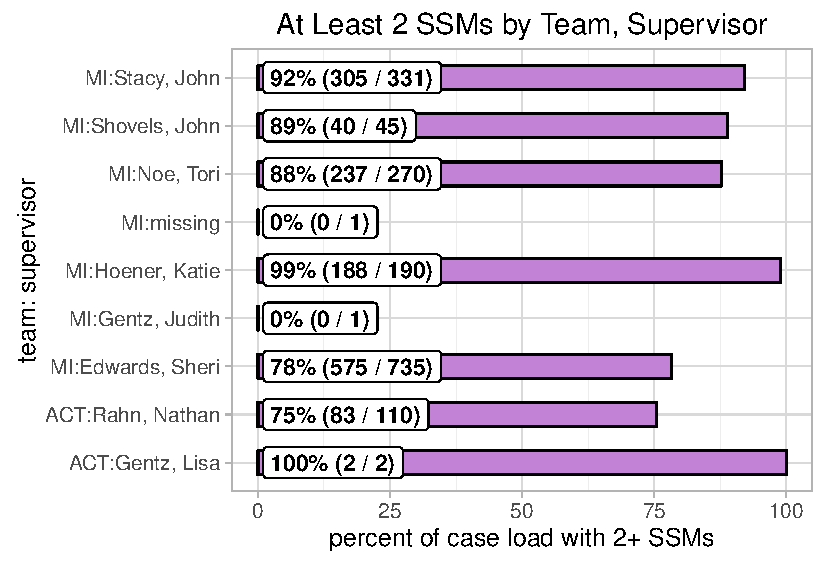
\includegraphics[width=\maxwidth]{figure/ssm_ts-1} 

\end{knitrout}

%' \pagebreak
%' <<ssm_tsa, fig.show="hold", message=FALSE, echo=FALSE, fig.height=5, fig.width=8>>=
%'
%' @
\end{document}
